\begin{filecontents}{apsrevcontrol.bib}
  @CONTROL{apsrev41Control,title="0"%,author="48",editor="1",pages="1",year="0"}
\end{filecontents}
\RequirePackage[l2tabu, orthodox]{nag}
\PassOptionsToPackage{pdftex,psdextra=true,
pdfversion=1.7,
pdfencoding=auto,
pdfnewwindow=true,
pdfusetitle=true,
%pdftitle={Inference vs. Influence},
%pdfauthor={E. Wolfe \& R.~W. Spekkens},
psdextra=true,
pdftoolbar=false,
pdfmenubar=false,
bookmarks=true,
bookmarksnumbered=true,
bookmarksopen=true,
pdfpagemode=UseThumbs,
bookmarksopenlevel=1,
pdfpagelabels=false
}{hyperref}
\documentclass[aps,english,superscriptaddress,twocolumn,twoside,longbibliography,prl,floatfix]{revtex4-1}%


\usepackage[utf8]{inputenx}% for arXiv use encoding ansinew
%\input{ix-utf8enc.dfu}
\usepackage[OT1]{fontenc}
\usepackage{amsfonts}
\usepackage{amssymb}
\usepackage{amsthm}
\usepackage{amsmath}
\usepackage{graphicx}%


\setcounter{MaxMatrixCols}{30}
\providecommand{\U}[1]{\protect\rule{.1in}{.1in}}
%EndMSIPreambleData
\newtheorem{theorem}{Theorem}
\newtheorem{acknowledgement}[theorem]{Acknowledgement}
\newtheorem{algorithm}[theorem]{Algorithm}
\newtheorem{axiom}[theorem]{Axiom}
\newtheorem{claim}[theorem]{Claim}
\newtheorem{conclusion}[theorem]{Conclusion}
\newtheorem{condition}[theorem]{Condition}
\newtheorem{conjecture}[theorem]{Conjecture}
\newtheorem{corollary}[theorem]{Corollary}
\newtheorem{criterion}[theorem]{Criterion}
\newtheorem{definition}[theorem]{Definition}
\newtheorem{example}[theorem]{Example}
\newtheorem{exercise}[theorem]{Exercise}
\newtheorem{lemma}[theorem]{Lemma}
\newtheorem{notation}[theorem]{Notation}
\newtheorem{problem}[theorem]{Problem}
\newtheorem{prop}{Proposition}
\newtheorem{taut}{Tautology}
\newtheorem{remark}[theorem]{Remark}
\newtheorem{solution}[theorem]{Solution}
\newtheorem{summary}[theorem]{Summary}
%\newenvironment{proof}[1][Proof]{\noindent\textbf{#1.} }{\ \rule{0.5em}{0.5em}}

% hyperlink stuff
\usepackage[usenames,dvipsnames]{color}
\definecolor{ultramarine}{RGB}{63, 0, 255}
\definecolor{medblue}{RGB}{0, 0, 100}
\definecolor{panblue}{RGB}{0,24,150}
\definecolor{carmine}{RGB}{150, 0, 24}
\usepackage[breaklinks=true]{hyperref}
\hypersetup{colorlinks,
linkcolor=carmine,
citecolor=medblue,
urlcolor=panblue,
anchorcolor=OliveGreen}
%\usepackage{url}


\definecolor{purple}{RGB}{128,0,128}
\newcommand{\purp}[1]{{\color{purple}{#1}\color{black}}}

\usepackage{verbatim} %for comment command
\usepackage{units}% for nicefrac
\newcommand{\half}[1]{\nicefrac{#1}{2}}

%\usepackage{braket} %provide \bra and \Bra and \set and \Set etc...
%\newcommand{\brackets}[1]{\lbrace{#1\rbrace}}
%\newcommand{\brackets}{\Set}



\usepackage{microtype}
\usepackage[capitalise]{cleveref}
\Crefname{eqs}{Eqs.}{Eqs.}
\creflabelformat{eqs}{(#2#1#3)}
\crefrangelabelformat{equation}{(#3#1#4-#5#2#6)}
%\crefmultiformat{equation}{eqs.~(#2#1#3)}{ and~(#2#1#3)}{, (#2#1#3)}{ and~(#2#1#3)}
\Crefmultiformat{equation}{Eqs.~(#2#1#3}{,#2#1#3)}{,#2#1#3}{,#2#1#3)}
\Crefname{prop}{\textbf{Prop}.}{\textbf{Props}.}
\Crefname{taut}{\textbf{Taut}.}{\textbf{Tauts}.}

\usepackage{mathtools} %for mathclap and prescript and more. Learning to love this package. And DeclarePairDelimeter!
\DeclarePairedDelimiter{\ceil}{\lceil}{\rceil}
\DeclarePairedDelimiter{\floor}{\lfloor}{\rfloor}
\DeclarePairedDelimiter{\parens}{\lparen}{\rparen}
\DeclarePairedDelimiter{\parenths}{\lparen}{\rparen}
\DeclarePairedDelimiter{\abs}{\lvert}{\rvert}
\DeclarePairedDelimiter{\norm}{\lVert}{\rVert}
\DeclarePairedDelimiter{\braces}{\lbrace}{\rbrace}
\DeclarePairedDelimiter{\bracks}{\lbrack}{\rbrack}
\newcommand{\brackets}[1]{\braces*{#1}}

%\usepackage{nath} %automatically pair delimiters. Provides \inline and \displayed. Adjusts \frac and /

\newcommand{\naf}{\ensuremath{\mathring{a}}}
\newcommand{\nbf}{\ensuremath{\mathring{b}}}
\newcommand{\ncf}{\ensuremath{\mathring{c}}}

\newcommand{\na}{\ensuremath{\lnot a}}
\newcommand{\nb}{\ensuremath{\lnot b}}
\newcommand{\nc}{\ensuremath{\lnot c}}

%\newcommand{\n}[1]{\ensuremath{\overline{#1}}}
\newcommand{\ot}[1]{\ensuremath{\overline{#1}}}
\newcommand{\Nor}[1]{\operatorname{\mathsf{Nor}}\!\bracks*{#1}}


\newcommand{\nap}{\ensuremath{a'}}
\newcommand{\nbp}{\ensuremath{b'}}
\newcommand{\ncp}{\ensuremath{c'}}
\newcommand{\napp}{\ensuremath{a''}}
\newcommand{\nbpp}{\ensuremath{b''}}
\newcommand{\ncpp}{\ensuremath{c''}}

\newcommand{\p}[1]{p\parenths*{#1}}
\newcommand{\cramp}[1]{\ensuremath{\mathord{#1}}}
\newcommand{\eql}{\cramp{=}}

\usepackage{bm}
\newcommand{\setlambda}{\bm{\lambda}}

%\newcommand{\cramp}[1]{\ensuremath{\mathopen{}#1\mathclose{}}}



\begin{document}
%\preprint{ }
%\title{Transitivity of implication and causal structure}
\title{Alternatives to Entropic Inequalities and the Triangle Scenario}
\author{Robert W. Spekkens}
\email{rspekkens@perimeterinstitute.ca}
\affiliation{Perimeter Institute for Theoretical Physics, Waterloo, Ontario, Canada, N2L 2Y5}
\author{Tobias Fritz}
\email{tfritz@perimeterinstitute.ca}
\affiliation{Perimeter Institute for Theoretical Physics, Waterloo, Ontario, Canada, N2L 2Y5}
\author{Elie Wolfe}
\email{ewolfe@perimeterinstitute.ca}
\affiliation{Perimeter Institute for Theoretical Physics, Waterloo, Ontario, Canada, N2L 2Y5}
\date{\today}


\begin{abstract}
Given some hypothesis of causal structure it is desirable to determine the set of probability distributions compatible with the hypothesis. For certain causal structures, such as Bell scenarios, the compatible set corresponds to the convex hull of various deterministic distributions, and admits a necessary and sufficient description in terms of conditional probability linear inequalities. For more general causal structures, however, it is far easier to derive entropic inequalities instead of probabilistic inequalities. Unfortunately there typically exist distributions which are genuinely incompatible with the causal structure but which satisfy all the structure's entropic inequalities. A tight characterization of all distributions which can be explained in terms of classical latent variables is critical in quantum information theory in order to recognize and exploit uniquely quantum distributions. The insufficiency of entropic inequalities, therefore, motivates us to explore alternative means of deriving compatibility tests for general causal structures, ideally directly at the level of probabilities. Uniquely quantum distributions are known to exist in the Triangle scenario; the methods presented herein may assist in isolating the criteria which distinguish quantum from classical distributions in that scenario.
\end{abstract}
\maketitle
%In Ref.~\cite{WoodSpekkens}, the standard proof of Bell's theorem is presented in the language of causal inference.  In particular, the CHSH inequality emerges as a special case of what Pearl calls an ``instrumental inequality''.  Hardy's proof of Bell's theorem is quite different from the standard proof and the following question naturally arises: is there a generic tool for classical causal inference of which the Hardy argument can be considered a special case when applied to the M-shaped causal structure of the Bell experiment?

%To try and answer this question, we apply Hardy-type reasoning to the triangle causal structure, that is, the one with three observed variables, each pair of which have a common cause.  We show that this sort of reasoning does indeed facilitate causal inference in the case of the triangle causal structure, thereby lending some evidence to the notion that this style of argument has the potential to be generalized into a generic tool for classical causal inference.

\section{Introduction}
***needs introduction, especially background and motivation.***


We follow the convention that upper-case letters indicate random variables while lower-case letters indicate some particular value associated with the corresponding random variable. In this convention, for example, a student's score on some test $T$ might depend probabilistically on the extent of sleep $S$. The Boolean proposition $T\cramp{=}t|S\cramp{=}s$ should be understood as "the students scores $t$ on the test given a duration of sleep equal to $s$. As conditional propositions form the basis of much of what follows, we introduce a natural shorthand based on subscripts, such as $t_s$ to indicate the proposition $T\cramp{=}t|S\cramp{=}s$. 

In the study of causal structures one often encounters hidden, or latent, variables, which are posited to explain apparent correlations and randomness. We'll use Greek letters to indicate latent random variables. Furthermore, we'll put a condition symbol ($|$) into the subscript to distinguish latent variables. Thus, $a_{x|\lambda}$ is the proposition $\parens*{A\cramp{=}a|X\cramp{=}x,\Lambda\cramp{=}\lambda}$. The use of explicit numbers can render this subscript notation ambiguous; we'll be define hard rules for interpreting numeric subscripts when they show up. 

Essential to our work here is that we can take the dependence on the latent variable to be deterministic. In other words,  $a_{x|\lambda}$ is always true or always false, and hence occurs with probability either zero or one. 

The deterministic dependence ensures that all joint probability terms involving latent variables automatically factor: $\p{a_{x|\lambda} , b_{y|\lambda}}=\p{a_{x|\lambda}}\p{b_{y|\lambda}}$, because binary multiplication is equivalent to logical conjunction. Indeed, the connection between formal logic statements and probabilities forms the essence of our technique for deriving inequalities.
%\begin{itemize}\setlength\itemsep{1em}
%  \item Conjunction  $\leadsto$ product of probabilities
%  \item Implication  $\leadsto$ $\p{\text{antecedent}}\leq\p{\text{consequent}}$
%  \item Exclusive Disjunction  $\leadsto$ sum of probabilities
%\end{itemize}
%\begin{itemize}\setlength\itemsep{1em}
%  \item $\bracks*{f_{1|\lambda} \land f_{2|\lambda}\land ...} \leadsto \bracks*{\p{a_{x|\lambda}}\p{b_{y|\lambda}}...=1}$
%  \item $\bracks*{f_{1|\lambda} \lor f_{2|\lambda} \lor ...} \leadsto \bracks*{\p{a_{x|\lambda}}+\p{b_{y|\lambda}}+...\geq 1}$
%\end{itemize}



%$\p{ab|xy\lambda}$ should be understood as ${\p{A\cramp{=}a,B\cramp{=}b|X\cramp{=}x,Y\cramp{=}y,\Lambda\cramp{=}\lambda}}$. 
%We use lower-case alphabetical subscripts to indicate conditioning upon a particular value, such that for instance $\p{a_x b_y|\lambda}=\p{ab|xy\lambda}$. 
We adopt the convention of indicating logical negation by $\operatorname{\mathsf{Not}}\!\bracks*{a}\equiv\na$ such that $\na$ references the possibility of \emph{any} outcome other than $a$, i.e. $\p{\na}\equiv\p{A\cramp{\neq}a}=1-\p{A\cramp{=}a}$. Note that Logical conjunction is herein represented by the use of commas, such that $\p{a,b}$ is the probability of $A\cramp{=}a$ \emph{and} $B\cramp{=}b$.

%We reserve the overbar notation, however, for negation as a form of constraint, such that $\ot{a}$ means \emph{some} particular outcome other than $a$, and hence $\p{\ot{a}}\leq \p{\na}$ etc. Only for the special case of binary $A$ do the the two forms of negation coincide, $\na=\ot{a}$. For multivalued variables we use the logical proposition $\Nor{a,\ot{a}}\equiv\lnot\parens*{a\lor \ot{a}}$ to reference the possibility of obtaining any outcome other than $a$ or $\ot{a}$, i.e. $\p{\Nor{a,\ot{a}}}=\p{A\cramp{\neq}a\land A\cramp{\neq}\ot{a}}$ and $\p{a}+\p{\na}+\p{\Nor{a,\ot{a}}}=1$.


\section{Hardy-Type Criteria Via Noncontextuality}

Per Ref.~[\citealp[]{LSW}, see also \citealp[]{H.Stapp:Hardy:Transitivity,D.Boschi:PRL:2755,Mermin,Unruh}], the Hardy-type proof of nonlocality~\cite{L.Hardy:PRL:1665} is fundamentally an expression of the the transitivity of implications among value assignments in noncontextual ontological models. Transitivity follows from noncontextuality because value assignments do not depend on the context (local or remote) of the measurement. Failure of the transitivity of implication therefore implies the impossibility of such models. We begin by recalling the Hardy paradox in this form, and then show how the assumption of transitivity can be replaced with the assumption of a particular causal structure. 

There are plenty of physical situation wherein the act of measurement cannot be accomplished without disturbing the system being measurement.  Thus for each instance where a pristine system is subject to analysis only one property of the system can be reliably probed. If such ``delicate" systems are being delivered to Alice and Bob then although they can make bipartite-simultaneous inquiries of various observables, nevertheless each party is restricted to examine only one of his or her local observables in a given trial. Let Alice's (Bob's) observables be $\brackets{A_0,A_1}$ ($\brackets{B_0,B_1}$).

Suppose after performing many trials Alice and Bob are confident in the measurement statistics that two events never occur:
\begin{align}\begin{split}\label{eq:hardydisjunctive}
\text{never }& \left[a_0,\nb_1\right],
\; \text{and never } \left[\na_1,b_0\right].
%\; \text{never } \left[a_1, b_1\right].
\end{split}\end{align}
Now, as every disjunctive is equivalent to a contrapositive, i.e.  $\lnot\parens*{p\land q}\iff p {\scriptstyle \implies} \lnot q$, one can re-express \cref{eq:hardydisjunctive} as
%For the purpose of discussion possible implication of these statistics it is convenient to re-express \cref{eq:hardydisjunctive}
%in an equivalent but contrapositive form, namely 
\begin{align}\begin{split}\label{eq:hardycontrapositive}
a_0 &{\scriptstyle \implies} b_1
\;\text{ and }\; b_0 {\scriptstyle \implies} a_1.
%\; b_1 {\scriptstyle \implies} \na_1.
\end{split}\end{align}

If, as presumed by noncontextual ontological models, measurement merely reveals a pre-existing value, then any given system must simultaneous possess the four objective \emph{properties} $\brackets{A_0,A_1,B_0,B_1}$ even though the fragility of the systems limits inquiry to one property per party per pristine instance. However, the special statistics per \cref{eq:hardydisjunctive} allow the experimenters to infer what Alice's and Bob's outcomes \emph{would} have been if they had measured $A_1$ and $B_1$, even though they \emph{actually} measured $A_0$ and $B_0$ and obtained $a_0$ and $b_0$ respectively. Accordingly, the set of systems with the properties $\left[a_0,b_0\right]$ must be a subset of the systems with the properties $\left[a_1,b_1\right]$, and therefore  \cref{eq:hardydisjunctive} implies that for noncontextual ontological models
\begin{align}
\left[a_0,b_0\right] {\scriptstyle \implies} \left[a_1,b_1\right].
\end{align}
and hence
%
%Now, if transitivity were to hold in \cref{eq:hardycontrapositive} then one could infer that 
%\begin{align}\label{eq:hardyimplication}
%a_0 &{\scriptstyle \implies} b_1 {\scriptstyle \implies} \na_1 {\scriptstyle \implies} \nb_0
%\end{align}
%where the final implication is via modus tollens. The composite implication $a_0 {\scriptstyle \implies} \nb_0 $ is equivalent to
\begin{align}\label{eq:hardyimplied}
%\text{ never }\left[a_0,b_0\right].
\p{a_0,b_0} \leq \p{a_1,b_1}.
\end{align}
%or back to disjunctive form, \cref{eq:hardydisjunctive} plus transitivity implies
%\begin{align}\label{eq:hardyimplicationdisjunctive}
%\text{never}&\quad \left[A_0,B_1\right].
%\end{align}
A heralded ramification of this conclusion is that the distribution known as the PR box~\cite{PROriginal,PRUnit}
\begin{align}\label{eq:PRbox}
p_{\text{PR}}\parens{a_x b_y}=\begin{cases}\tfrac{1}{2}&\text{if }\; a\oplus b= x y \\ 0&\text{otherwise}\end{cases},
\end{align}
where $a,b,x,y\in\brackets{0,1}$,
is incompatible with noncontextual ontological models, because it satisfies \cref{eq:hardydisjunctive} but not \cref{eq:hardyimplied}. 
%Note that in \cref{eq:PRbox} we have employed the shorthand 
%\begin{align}\label{eq:allbutone}
%a^{\prime}=\begin{cases} 1 &\text{if }a=1 \\ 0 & \text{if }a\neq 1\end{cases}
%\end{align}
%etc.

\section{Hardy Criteria Via Causal Inference}
\purp{This section has been rewritten, now using the tautology-to-inequality formalism, to link to Fritz's method.}

%It is often claimed that classically one must have $\p{a_1 b_1}\geq \p{a_0 b_0}$ from just the first two conditions in  \cref{eq:hardycontrapositive} alone \cite{CabelloHardyInequality}, such that the result ``If additionally $\p{a_1 b_1}=0$ then $\p{a_0 b_0}=0$" is just a special case. 
We now demonstrate that this Hardy-type inequality follows naturally from assumptions about causal structure. More importantly, we show that Hardy-type arguments can be used to derive compatibility criteria in the same vein even for general causal structures.

\begin{figure}[t!]
 \center{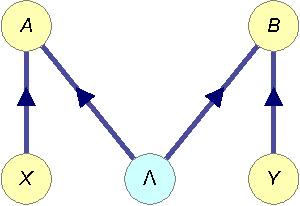
\includegraphics[width=2in]{BellDAGcap.pdf}}
\caption{The causal structure of the Bell scenario, on which Bell's theorem is based.}
 \label{fig:BellDAG}
\end{figure}

Consider the causal structure associated to the Bell experiment, depicted in \cref{fig:BellDAG}. $\brackets{A,B,X,Y}$ are all observable variables whereas $\lambda$ is the latent common cause of $A$ and $B$.

%Without loss of generality let's assume that the values $\Lambda\mathopen{=}\lambda$ are drawn from some (possibly infinite, possibly continuous) set $\lambda\in\Omega$. 
The assumption of causal structure dictates that
\begin{align}\begin{split}\label{eq:bellstructure}
\p{a,b|x,y,\lambda}=\p{a_{x|\lambda}}\p{b_{y|\lambda}}
\end{split}\end{align}
and accordingly that
\begin{align}\begin{split}\label{eq:bellintegration}
&\p{a_x b_y}
=\int\limits_{\mathclap{\text{all }\lambda}}\p{a_{x|\lambda}}\p{b_{y|\lambda}}\p{\lambda}.
\end{split}\end{align}



Now, any implicative condition between variables, such as those in \cref{eq:hardycontrapositive},  can be understood as statements regarding the the common parent of the variables. Any correlation between variables which do not influence each other requires an explanation in terms of a common cause, and $a_x {\scriptstyle \implies} b_y$ is certainly a non-trivial correlation. Thus $a_x {\scriptstyle \implies} b_y$ means that whenever $\Lambda=\lambda$ gives rise to $a_x$ it must be that $\lambda$ also gives rise to $b_y$. 

\textbf{Notation key:} When discussing the Bell scenario, let the first subscript on ``$a$" always stand for $x$, and similarly $y$ for ``$b$". Thus ${a_i \equiv \parens*{A\cramp{=}a|X\cramp{=}i}}$ and ${b_i \equiv \parens*{B\cramp{=}b|Y\cramp{=}i}}$ etc.


%Without loss of generality we may treat the dependence on the latent variable as deterministic, such that $\bracks*{a_0|\lambda}$ refers to the event wherein $A\cramp{=}a$ with probability one whenever $X\cramp{=}0$ and $\Lambda\cramp{=}\lambda$. Deterministic dependence allows us to translate observable inferences into conditional-probability inequalities, such that $a_0 {\scriptstyle \implies} b_1$ can be recast into $\forall_{\lambda}\;\p{a_0|\lambda}\leq \p{b_1|\lambda}$.


The tautology
\begin{taut}\label{taut:Hardy}The following is tautologically true:
%\begin{align*}
%\text{if }&\;\; \p{a_0|\lambda}\leq\p{b_1|\lambda},\\
%\text{and }&\;\; \p{b_0|\lambda}\leq\p{a_1|\lambda},\\
%\text{then }&\;\; \p{a_0|\lambda}\p{b_0|\lambda}\leq\p{a_1|\lambda}\p{b_1|\lambda}.
%\end{align*}
\begin{align*}
\text{if }&\;\; a_{0|\lambda} {\scriptstyle \implies} b_{1|\lambda},\\
\text{and }&\;\; b_{0|\lambda} {\scriptstyle \implies} a_{1|\lambda},\\
\text{then }&\;\; \p{a_0|\lambda}\p{b_0|\lambda}\leq\p{a_1|\lambda}\p{b_1|\lambda},\\
\text{since then }&\;\; \parens*{a_{0|\lambda} , b_{0|\lambda}} {\scriptstyle \implies} \parens*{a_{1|\lambda} , b_{1|\lambda}}.
\end{align*}
\end{taut}
%\begin{align}
%\text{if when }&\Lambda\cramp{=}\lambda:\;\; \bracks*{a_0|\lambda} {\scriptstyle \implies} \bracks*{b_1|\lambda},\label{eq:A0impB1alt}\\
%\text{and when }&\Lambda\cramp{=}\lambda:\;\; \bracks*{b_0|\lambda} {\scriptstyle \implies} \bracks*{a_1|\lambda},\label{eq:B0impA1alt}\\
%\text{ then }&\;\; \bracks*{a_0 b_0|\lambda} {\scriptstyle \implies} \bracks*{a_1 b_1|\lambda} .
%\end{align}
%\begin{align}
%{\rm if  }\;\; &\bracks*{a_0|\lambda} {\scriptstyle \implies} \bracks*{b_1|\lambda},\label{eq:A0impB1alt}\\
%{\rm and }\;\; &\bracks*{b_0|\lambda} {\scriptstyle \implies} \bracks*{a_1|\lambda},\label{eq:B0impA1alt}\\
%{\rm then }\;\; &\bracks*{a_0 b_0|\lambda} {\scriptstyle \implies} \bracks*{a_1 b_1|\lambda} .
%\end{align}
\noindent explains how the correlation $a_x {\scriptstyle \implies} b_y$ might come about. If the first two conditions of  \cref{taut:Hardy} are effectively verified for \emph{all} $\lambda$ (in that no exception is ever noticed) then the corresponding conclusion holds true for all $\lambda$. 

By integrating \cref{taut:Hardy} pursuant to \cref{eq:bellintegration} we obtain the desired inference, namely




%$\Lambda$, in the sense that, say, any $\lambda$ which gives rise to $a_0$ must -- with probability 1 -- also give rise to $b_1$. Formally, ``$a_0$ implies $b_1$" is equivalent to ``$\forall_\lambda\!:\;\text{if }\p{a_0|\lambda}\neq 0 \text{ then }\p{b_1|\lambda}=1$". This inequality, together with the causal structure implication of \cref{eq:bellintegration}, leads to



\begin{prop} \label{prop:BellNoGo}
The Bell causal structure (\cref{fig:BellDAG}) implies
\begin{align*}
\text{if  }\;\; \p{a_0 b_1}&=\p{a_0},\\
\text{and }\;\; \p{a_1 b_0}&=\p{b_0},\\
\text{then }\;\; \p{a_0 b_0}&\leq \p{a_1 b_1}.
\end{align*}
\end{prop}

The proposition follows from the tautology via
\begin{align}
\int_{\lambda}\p{a_{0|\lambda}}\p{b_{0|\lambda}}\p{\lambda} \leq \int_{\lambda}\p{a_{1|\lambda}}\p{b_{1|\lambda}}\p{\lambda}.
\end{align}


\begin{comment}
\begin{proof}
Note that \cref{eq:A0impB1source,eq:B0impA1source} are understood in terms of the latent variable as
\begin{align}
&\forall_{\lambda}\; %=
\p{b_1|\lambda}\geq \p{a_0|\lambda} ,\label{eq:A0eqB1}
\\&\forall_{\lambda}\; 
\p{b_0|\lambda}\geq \p{a_1|\lambda}.\label{eq:B0eqA1}
%\\&\exists_{\lambda_*} {\lambda_* \in \Omega_*}
%\exists_{\lambda_*}\; \p{\lambda_*}>0,\;\p{\left[A_0\right]||\lambda_*}>0,\;\p{\left[B_0\right]||\lambda_*}>0
%,\label{eq:A0B0pos}
\end{align}
Substitution into \cref{eq:bellintegration} then implies
\begin{align}\begin{split}\label{eq:hardyintegrals}
\p{a_0 b_0}&=\int_\lambda%\limits_{\mathclap{\text{all }\lambda}}
\p{a_0|\lambda}\p{b_0|\lambda}\p{\lambda}\\
%&=\int\limits_{\mathclap{\lambda\in \Omega{\left[a_0 b_0\right]}}} \p{a_0|\lambda}\p{b_0|\lambda}\p{\lambda}\\
&\leq \int_\lambda%\limits_{\mathclap{\text{all }\lambda}}
\p{b_1|\lambda}\p{a_1|\lambda}\p{\lambda}\\
%&\leq\int\limits_{\mathclap{\lambda\in \Omega}} \p{b_1|\lambda}\p{a_1|\lambda}\p{\lambda}\\
&=\p{a_1 b_1}\qedhere
\end{split}\end{align}
%The idea which converts this argument into something practical, i.e. upgrades \cref{eq:hardyintegrals} into Prop.~\ref{prop:BellNoGo}, is that deterministic relationships between observed variables are equivalent to For-All statements regarding their common causes under the assumption of causal structure.
%
%In our example, \cref{eq:A0eqB1,eq:B0eqA1} are derivable from the observable statistics posited in \cref{eq:A0impB1source,eq:B0impA1source} respectively. \cref{eq:A0eqB1,eq:B0eqA1} follow from \cref{eq:A0impB1source,eq:B0impA1source} because any $\lambda$ which even occasionally gives rise to $a_0$ must also certainly give rise to $b_1$ as the observable statistics prohibit the events $\left[a_0,\nb_1\right]$ or $\left[\na_1,B_0\right]$.
%To be clear, if $\p{a_0|\lambda}=0$ then the \cref{eq:A0impB1source} is thoroughly uninformative regarding $\p{b_1|\lambda}$, as any such $\lambda$ is excluded from consideration in \cref{eq:A0eqB1}.
\end{proof}
\end{comment}

\section{Inequalities from Tautologies}
By examining further tautologies in terms of the latent variable we can obtain even stronger results. For example, consider the binary-multiplication tautology
%\begin{align}
%\bracks*{a_0 b_0|\lambda} \implies \bracks*{a_0 b_1|\lambda} \lor \bracks*{a_1 b_0|\lambda} \lor \bracks*{\na_1 \nb_1|\lambda}
%\text{if  when }&\Lambda\cramp{=}\lambda:\;\; \bracks*{a_0 b_0|\lambda},\\
%\text{then }&\;\; \bracks*{a_0 b_1|\lambda} \lor \bracks*{a_1 b_0|\lambda} \lor \bracks*{\na_1 \nb_1|\lambda}
%\end{align}
\begin{taut}\label{taut:CH}The following is tautologically true:
\begin{align*}
&\p{a_{0|\lambda}} \p{b_{0|\lambda}}\leq
\\& \p{a_{0|\lambda}}\p{\nb_{1|\lambda}} + \p{\na_{1|\lambda}}\p{b_{0|\lambda}} + \p{a_{1|\lambda}}\p{b_{1|\lambda}}
%\text{if }\;\; \p{a_0|\lambda}\p{b_0|\lambda}&=1,\\
%\text{then }\;\; \p{a_1|\lambda}\p{b_1|\lambda}&=1,\\
%\text{or }\;\; \p{\na_1|\lambda}\p{b_0|\lambda}&=1,\\
%\text{or }\;\;\p{a_0|\lambda}\p{\nb_1|\lambda}&=1.
\end{align*}
\end{taut}
\noindent which follows from the logical-disjunction tautology
\begin{align}\begin{split}\label{eq:CHtautraw}
%&\parens*{a_{0|\lambda} \land b_{0|\lambda}} \implies\\& \parens*{a_{0|\lambda} \land \nb_{1|\lambda}} \lor \parens*{b_{0|\lambda} \land \na_{1|\lambda}} \lor \parens*{a_{1|\lambda} \land b_{1|\lambda}}.
&\parens*{a_{0|\lambda} , b_{0|\lambda}} \implies\\& \parens*{a_{0|\lambda} , \nb_{1|\lambda}} \bigvee \parens*{b_{0|\lambda} , \na_{1|\lambda}} \bigvee \parens*{a_{1|\lambda} , b_{1|\lambda}}.
\end{split}\end{align}
Integrating both sides of \cref{taut:CH} according to \cref{eq:bellintegration} implies the unconditional inequality
\begin{align}\label{eq:CHraw}
%\p{a_0 b_0|\lambda}\leq \p{a_0 \nb_1|\lambda} + \p{\na_1 b_0|\lambda} + \p{a_1,b_1|\lambda}
{\p{a_0 b_0} \leq \p{a_0 \nb_1} + \p{\na_1 b_0} + \p{a_1,b_1}}.
\end{align}
%and hence teaches us the unconditional inequality ${\p{a_0 b_0} \leq \p{a_0 \nb_1} + \p{\na_1 b_0} + \p{a_1,b_1}}$, which 
Finally, by substituting $\p{a_0 \nb_1} \to \p{a_0}-\p{a_0 b_1}$ etc, \cref{eq:CHraw} is seen to be precisely the CH inequality! Thus we have
\begin{prop} \label{prop:CH}
The Bell causal structure (\cref{fig:BellDAG}) implies
\begin{align*}
%&\p{a_0 b_0} \leq \p{a_0 \nb_1} + \p{\na_1 b_0} + \p{a_1,b_1}
%\\&\text{or, letting }\;\; \p{a_0 \nb_1} \to \p{a_0}-\p{a_0 b_1}\;\text{ etc,}
%\\&\p{a_0 b_0} +\p{a_0 b_1} + \p{a_1 b_0} - \p{a_1,b_1} -\p{a_0} - \p{b_0} \leq 0
\\&\p{a_0 b_0} +\p{a_0 b_1} + \p{a_1 b_0} \leq \p{a_1,b_1} +\p{a_0} + \p{b_0}
\end{align*}
\end{prop}
\noindent which implies \cref{prop:BellNoGo} as a special case.


Note that \cref{taut:Hardy} and \cref{taut:CH} are directly related. \cref{taut:Hardy} can be recast as a ``destructive dilemma", namely
\begin{align}\begin{split}
&\parens*{a_{0|\lambda} {\scriptstyle \implies}  b_{1|\lambda}} \bigwedge \parens*{b_{0|\lambda} {\scriptstyle \implies}  a_{1|\lambda}} \bigwedge \parens*{\na_{1|\lambda} \lor \nb_{1|\lambda}}\\ &\implies \parens*{\na_{0|\lambda} \lor \nb_{0|\lambda}}
\end{split}\end{align}
which is the contraposition of \cref{eq:CHtautraw}.
%whereas \cref{taut:CH} is its contrapositive, namely 
%\begin{align}\begin{split}
%&\parens*{a_0 \land b_0|\lambda} \implies\\& \parens*{a_0 \land \nb_1|\lambda} \lor \parens*{b_0 \land \na_1|\lambda} \lor \parens*{a_1 \land b_1|\lambda}.
%\end{split}\end{align}
%In this derivation, the tautology is rexpressed 
%\begin{align}
%\bracks*{a_0 b_0|\lambda} \implies \bracks*{a_0 b_1|\lambda} \lor \bracks*{a_1 b_0|\lambda} \lor \bracks*{\na_1 \nb_1|\lambda}
%\text{if  when }&\Lambda\cramp{=}\lambda:\;\; \p{a_0|\lambda}\p{b_0|\lambda}=1,\\
%\text{then }&\;\; \p{a_0|\lambda}\p{b_1|\lambda}=1\\
%\text{or }&\;\; \p{a_1|\lambda}\p{b_0|\lambda}=1\\
%\text{or }&\;\;p{\na_1|\lambda}\p{\nb_1|\lambda}=1\\
%\text{so surely }&\;\;\p{a_0 b_0|\lambda}\leq \p{a_0 b_1|\lambda} + \p{a_1 b_0|\lambda} + \p{\Nor{a_1,b_1|\lambda}}\\
%\end{align}


\section{The triangle causal structure}

The same causal inference logic can be applied to the Triangle scenario, namely the causal structure depicted in \cref{fig:TriDAG}. Here $\brackets{A,B,C}$ and the observed variables, and  $\brackets{\Lambda_{AB},\Lambda_{BC},\Lambda_{AC}}$ are latent. $\Lambda_{AB}$ denotes the common cause of $A$ and $B$, etc. 


\begin{figure}[!t]
 \center{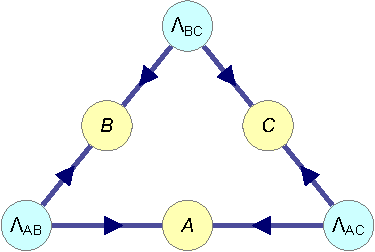
\includegraphics[width=2.5in]{TriDAGcap.pdf}}
\caption{The causal structure of the Triangle scenario, for which the three observed variables lack a common ancestor.}
 \label{fig:TriDAG}
\end{figure}


The Triangle scenario's causal structure dictates that
\begin{align}\begin{split}\label{eq:tristructure}
p&\parens{abc|\lambda_{AB}\lambda_{BC}\lambda_{AC}}\\
&=\p{a|\lambda_{AC}\lambda_{AB}}\p{b|\lambda_{AB}\lambda_{BC}}\p{c|\lambda_{BC}\lambda_{AC}}.
\end{split}\end{align}
%For excessive clarity, let $\Omega_{AB}\left[\_\_\right]$ denote the complete set of values which $\lambda_{AB}$ can take, and let $\Omega_{AB}\left[a\_\right]$ denote the special subset of possible $\lambda_{AB}$ for which ${\p{a|\lambda_{AB}}\neq 0}$. %$\exists_{\lambda_{AC}}\!:\; {\p{a|\lambda_{AB}\lambda_{AC}}>0}$.
Accordingly,
\begin{align}\label{eq:triintegration}
&\p{abc}=\\\nonumber
&\iiint\limits_{\mathclap{\lambda_{AB}\lambda_{BC}\lambda_{AC}}}\,
%&\int\!\!\int\limits_{\mathclap{\lambda_{AB}\lambda_{BC}\lambda_{AC}}}\!\!\int
%\limits_{\mathclap{\substack{\lambda_{AB}\in \Omega_{AB}\left[\_\_\right]\\\lambda_{BC}\in \Omega_{BC}\left[\_\_\right]\\\lambda_{AC}\in \Omega_{AC}\left[\_\_\right]}}}
\begin{pmatrix}\p{a_{|\lambda_{AC}\lambda_{AB}}}\p{b_{|\lambda_{AB}\lambda_{BC}}}\p{c_{|\lambda_{BC}\lambda_{AC}}}\\
\times \p{\lambda_{AB}}\p{\lambda_{BC}}\p{\lambda_{AC}}\end{pmatrix}.
\end{align}
There is no reason for us to consider specific values of a hidden random variable. As such, we'll use numbers to \emph{index} latent variable, and not to imagine them taking on specific values.

\textbf{Notation key:}  When discussing the Triangle scenario, let the two indices of $k_{|ij}$ refer to the two parental latent variables of $K$ in \emph{clockwise} order as they appear in \cref{fig:TriDAG}. Thus ${a_{|ij} \equiv \parens*{
A\cramp{=}a|\Lambda_{AC}\cramp{=}\lambda_{AC}^{(i)},\Lambda_{AB}\cramp{=}\lambda_{AB}^{(j)}}}$ and ${b_{|ij} \equiv \parens*{B\cramp{=}b|\Lambda_{AB}\cramp{=}\lambda_{AB}^{(i)},\Lambda_{BC}\cramp{=}\lambda_{BC}^{(j)}}}$ , etc.

%As the triangle scenario has more than one latent variable, it becomes important to imagine independent and identically distributed sets of each latent variable, such that $\p{\Lambda_{AB}^{(1)}\cramp{=}\lambda_{AB}^{(1)},\Lambda_{AB}^{(2)}\cramp{=}\lambda_{AB}^{(2)}}=\p{\Lambda_{AB}\cramp{=}\lambda_{AB}^{(1)}}\p{\Lambda_{AB}\cramp{=}\lambda_{AB}^{(2)}}$. Let $\p{b_{|ij}}$ denote $\p{b|\lambda_{AB}^{(i)}\lambda_{BC}^{(j)}}$ and let $\p{a_{|ij}}$ denote $\p{a|\lambda_{AC}^{(i)}\lambda_{AB}^{(j)}}$, such that the two indices of $k_{|ij}$ refer to the two parental latent variables of $K$ in \emph{clockwise} order as they appear in \cref{fig:TriDAG}.






As with the Bell scenario, we can derive unconditional inequalities by considering tautologies based on the principle of the excluded middle. For example,
\begin{taut}\label{taut:FritzF2}The following is tautologically true:
\begin{align*}
\begin{split}
&\p{a_{|11}}\p{b_{|22}}\p{c_{|33}}\leq\\& \p{{a'}_{|31}}\p{{b'}_{|12}}\p{{c'}_{|23}} + \p{a_{|11}}\p{{\nb'}_{|12}} \\&+ \p{b_{|22}}\p{{\nc'}_{|23}} + \p{c_{|33}}\p{{\na'}_{|31}}
\end{split}
%\text{if }\;\; \p{a_{11}}\p{b_{22}}\p{c_{33}}&=1,\\
%\text{then }\;\; \p{a'_{31}}\p{b'_{12}}\p{c'_{23}}&=1\\
%\text{or }\;\; \p{a_{11}}\p{\nb'_{12}}&=1\\
%\text{or }\;\; \p{b_{22}}\p{\nc'_{23}}&=1\\
%\text{or }\;\; \p{c_{33}}\p{\na'_{31}}&=1
\end{align*}
\end{taut}
follows from the logical-disjunction tautology 
\begin{align}\begin{split}
%\p{a_{11}}&\p{b_{22}}\p{c_{33}}\leq\\& \p{a'_{31}}\p{b'_{12}}\p{c'_{23}} + \p{a_{11}}\p{\nb'_{12}} \\+& \p{b_{22}}\p{\nc'_{23}} + \p{c_{33}}\p{\na'_{31}}
&\parens*{a_{|11},b_{|22},c_{|33}}\implies\\& \parens{{a'}_{|31},{b'}_{|12},{c'}_{|23}} \bigvee \parens{a_{|11},{\nb'}_{|12}} \\&\bigvee \parens{b_{|22},{\nc'}_{|23}} \bigvee \parens{c_{|33},{\na'}_{|31}}
\end{split}\end{align}
and hence teaches us the unconditional inequality
\begin{prop} \label{prop:FritzF2}
The Triangle causal structure (\cref{fig:TriDAG}) implies that, for any $\brackets{\nap,\nbp,\ncp}$,
\begin{align*}\begin{split}
\p{a}&\p{b}\p{c}\leq\\& \p{a'b'c'} + \p{a\nb'} + \p{b\nc'} + \p{c\na'}.
\end{split}\end{align*}
\end{prop}

The causal structure is employed in going from \cref{taut:FritzF2} to \cref{prop:FritzF2}, in the sense of using \cref{eq:triintegration}.


%which implies \cref{prop:TriNoGo} as a special case.
%\purp{EDITING...}
%As before, \cref{taut:Spekkens} and \cref{taut:FritzF2} are directly related. \cref{taut:Spekkens} can be recast in conjunctive form as
%\begin{align}\begin{split}
%&\parens*{\na_{11} \lor b'_{12}} \land \parens*{\nb_{22} \lor c'_{23}} \\&\land \parens*{\nc_{33} \lor a'_{31}}\land\parens*{\na'_{31} \lor \nb'_{12} \lor \nc'_{23}}  \\&\implies \parens*{\na_{11} \lor \nb_{22} \lor \nc_{33}}
%\end{split}\end{align}
%whereas \cref{taut:FritzF2} is its contrapositive, namely 
%\begin{align}\begin{split}
%&\parens*{a_{11} \land b_{22} \land c_{33}} \implies\\& \parens*{a'_{31} \land b'_{12} \land c'_{23}} \lor \parens*{a_{11} \land \nb'_{12}} \\&\lor \parens*{b_{22} \land \nc'_{23}|\lambda} \lor \parens*{c_{33} \land \na'_{31}}.
%\end{split}\end{align}



When we integrate the final inequality in \cref{taut:FritzF2} we find that the causal structure treats the two sides of the inequality quite differently. The left-hand-side \emph{factors}, namely
\begin{align*}
&\int_{\setlambda}\,
\begin{pmatrix}
\p{a_{|\lambda_{AB}^{(1)}\lambda_{AC}^{(1)}}}
\\\times \p{b_{|\lambda_{AB}^{(2)}\lambda_{BC}^{(2)}}}
\\\times \p{c_{|\lambda_{BC}^{(3)}\lambda_{AC}^{(3)}}}
\\\times \p{\lambda_{AB}^{(1)}}\p{\lambda_{BC}^{(1)}} \p{\lambda_{AC}^{(1)}}
\\\times \p{\lambda_{AB}^{(2)}}\p{\lambda_{BC}^{(2)}} \p{\lambda_{AC}^{(2)}}
\\\times \p{\lambda_{AB}^{(3)}}\p{\lambda_{BC}^{(3)}} \p{\lambda_{AC}^{(3)}}.
\end{pmatrix}=
\\&\begin{pmatrix}
\int_{\setlambda}\,\p{a_{|11}}\p{\lambda_{AB}^{(1)}\lambda_{AC}^{(1)}}
\\\times \int_{\setlambda}\,\p{b_{|22}}\p{\lambda_{AB}^{(2)}\lambda_{BC}^{(2)}}
\\\times \int_{\setlambda}\,\p{c_{|33}}\p{\lambda_{BC}^{(3)}\lambda_{AC}^{(3)}}
\end{pmatrix}=\p{a}\p{b}\p{c}.
%\\&\parens*{\int_{\setlambda}\,\p{a_{|11}}\p{\lambda_{AB}^{(1)}\lambda_{AC}^{(1)}}}\parens*{\int_{\setlambda}\,\p{b_{|22}}\p{\lambda_{AB}^{(2)}\lambda_{BC}^{(2)}}}...
%\\&\int_{\setlambda}\,\p{a_{|11}}\p{b_{|22}}\p{c_{|33}}\p{\lambda_{AB}^{(1)}\lambda_{AC}^{(1)}\lambda_{AB}^{(2)}\lambda_{BC}^{(2)}\lambda_{BC}^{(3)}\lambda_{AC}^{(3)}}
%\\&=\p{a}\p{b}\p{c}
\end{align*}
The terms on the right-hand-side do not factor, however; namely
\begin{align*}
\int_{\setlambda}\,\p{{a'}_{|31}}\p{{b'}_{|12}}\p{{c'}_{|23}}\p{\lambda_{AB}^{(1)}\lambda_{BC}^{(2)}\lambda_{AC}^{(3)}}=\p{a' b' c'}
\end{align*}
%\begin{align*}
%\int_{\setlambda}\,
%\begin{pmatrix}
%\p{{a'}_{|\lambda_{AB}^{(1)}\lambda_{AC}^{(3)}}}
%\\\times \p{{b'}_{|\lambda_{AB}^{(1)}\lambda_{BC}^{(2)}}}
%\\\times \p{{c'}_{|\lambda_{BC}^{(2)}\lambda_{AC}^{(3)}}}
%\\\times \p{\lambda_{AB}^{(1)}}\p{\lambda_{BC}^{(1)}} \p{\lambda_{AC}^{(1)}}
%\\\times \p{\lambda_{AB}^{(2)}}\p{\lambda_{BC}^{(2)}} \p{\lambda_{AC}^{(2)}}
%\\\times \p{\lambda_{AB}^{(3)}}\p{\lambda_{BC}^{(3)}} \p{\lambda_{AC}^{(3)}}
%\end{pmatrix}=\p{a' b' c'},
%\end{align*}
and 
\begin{align*}
\int_{\setlambda}\,\p{a_{|11}}\p{{\nb'}_{|12}}\p{\lambda_{AB}^{(1)}\lambda_{BC}^{(2)}\lambda_{AC}^{(1)}}=\p{a\nb'}
\end{align*}
etc.


\begin{comment}
Accounting for the causal structure, then, the implication of \cref{taut:Spekkens} is
\begin{prop} \label{prop:TriNoGo}
The Triangle causal structure (\cref{fig:TriDAG}) implies that, for any $\brackets{\nap,\nbp,\ncp}$,
\begin{align}
{\rm if  }\;\; &\p{a\, b'}=\p{a},\label{eq:AimpNotBsource}\\
{\rm and }\;\; &\p{b\, c'}=\p{b},\label{eq:BimpNotCsource}\\
{\rm and }\;\; &\p{c\, a'}=\p{c},\label{eq:CimpNotAsource}\\
{\rm then }\;\; &\p{a}\p{b}\p{c}\leq \p{a' b' c'}.\label{eq:spekkensresult}
\end{align}
%As $\p{abc}\geq \p{a}\p{b}\p{c}$ for any causal structure, the proposition is strongest when $a\neq a'$ etc.
\end{prop}
\end{comment}

A consequence of Prop.~\ref{prop:FritzF2} is that the W-type distribution
\begin{align}\label{eq:wdistribution}
p_{\text{W}}\parens{abc}=\begin{cases}\tfrac{1}{3}&\text{if }\; a+b+c=1 \\ 0&\text{otherwise}\end{cases}
\end{align}
is found to be incompatible with the Triangle scenario, where $a,b,c\in\brackets{0,1}$. The W-distribution states that the in any event in which $A,B,C$ are observed, precisely one of them will be found to equal $1$ while the other two will equal $0$. The identity of the variable which takes the value $1$ is uniformly random. 
To see how this distribution is incompatible with Prop.~\ref{prop:FritzF2}, note that for three \emph{identical} (but not independent) binary variables a special case of Prop.~\ref{prop:FritzF2} is
\begin{align*}\begin{split}
3\times\p{A\cramp{=}0}&\leq \p{A\cramp{=}B\cramp{=}C\cramp{=}1} + 3\times\p{A\cramp{=}0,B\cramp{=}0}.
\end{split}\end{align*}
For the W-distribution $\p{A\cramp{=}0}=\nicefrac{2}{3}$, $\p{A\cramp{=}B\cramp{=}C\cramp{=}1}=0$, and $\p{A\cramp{=}0,\cramp{=}0}=\nicefrac{1}{3}$, hence incompatible.


%The W-distribution conflicts with Prop.~\ref{prop:TriNoGo} because ${p_{\text{W}}\parens{10\_}}={p_{\text{W}}\parens{1\_\_}}={p_{\text{W}}\parens{\_10}}={p_{\text{W}}\parens{\_1\_}}={p_{\text{W}}\parens{0\_1}}={p_{\text{W}}\parens{\_\_1}}{=\nicefrac{1}{3}}$ but ${p_{\text{W}}\parens{111}}=0$.%<\nicefrac{1}{3}$. 

\section{Failure of Entropic Inequalities}

It is interesting to note that entropic inequalities \cite{fritz2013marginal,chaves2014novel} fail to recognize the PR-box as incompatible with the Bell scenario and also the W-type distribution as incompatible with the Triangle scenario, whereas Hardy-type reasoning is capable of doing so. To reiterate from the abstract, enumeration of entropic inequalities is considered state-of-the-art derivation of necessary albeit insufficient causal structure compatibility criteria \cite{pusey2014gdag}. The insufficiency is a pressing concern in quantum information theory as there are uniquely-quantum distributions which cannot be certified as non-classical by means of entropic inequalities \cite{fritz2012bell}. 

The entropic inequalities associated with the Bell scenario\footnote{Generally a non-trivial entropic inequality is defined as one that takes into account the causal structure somehow. There are no such entropic inequalities for Bell scenarios, so the inequality listed here is Shannon-type, and can be derived from nothing more than the assumption of joint measurability.} are given by
\begin{align}\begin{split}\label{eq:entropicCHSH}
&H\parens{A_1,B_1}+H\parens{A_0}+H\parens{B_0}
\\&\leq H\parens{A_0,B_0}+H\parens{A_0,B_1}+H\parens{A_1,B_0}
\end{split}\end{align}
and its permutations \cite{chaves2014novel,chaves2012entropic}.

The entropic inequalities associated with the Triangle scenario are given by 
\begin{align}\begin{split}\label{eq:entropicineqs}
&I\parens{A:B}+I\parens{A:C}\leq H\parens{A} \\
\text{and }\quad&I\parens{A:B}+I\parens{A:C}+I\parens{B:C}\\
& \leq H\parens{A,B}-I\parens{A:B:C}\\
\text{and }\quad & I\parens{A:B}+I\parens{A:C}+I\parens{B:C}
\\& \leq\frac{H\parens{A}+H\parens{B}+H\parens{C}}{2}-I\parens{A:B:C}
\end{split}\end{align}
and their permutations \cite{chaves2014novel,Chaves2015infoquantum,pusey2014gdag}.

Note that bipartite mutual information may be understood as $I\parens{A:B}\equiv H\parens{A}+H\parens{B}-H\parens{A,B}$ and tripartite mutual information is defined as $I\parens{A:B:C}\equiv H\parens{A}+H\parens{B}+H\parens{C}-H\parens{A,B}-H\parens{A,C}-H\parens{B,C}+H\parens{A,B,C}$. It is straightforward to demonstrate that the distributions given in \cref{eq:PRbox,eq:wdistribution} satisfy  \cref{eq:entropicCHSH,eq:entropicineqs} respectively.



\section{Deriving Polynomial Inequalities}

\purp{Requires re-writing, in-lou of basic method and notation introduced earlier. This section will become about \emph{strengthening} unconditional tautologies, and deriving them algorithmically.\\}

We have seen that certain tautologies involving deterministic response functions (probabilities conditioned on values of the latent variables) can be translated into polynomial inequalities by integration. We now seek to formalize an algorithm for the development of such polynomial inequalities for general causal structures.

There are only two rules: First, the tautology must be logically closed. 

Second, the tautology must involve only products of response functions which admit integration.
Thus, for example, terms like $\p{a_{|22}}\p{{\nb'}_{|23}}\p{{a''}_{|11}}\p{c_{|11}}$ are acceptable, whereas terms like $\p{a_{|12}}\p{b_{|21}}\p{c_{|12}}$ are not allowed. In a disallowed product, the same latent variable appears referenced with different indices. In the aforementioned example, to make
\begin{align}
\p{a|\lambda^{(1)}_{AC}\lambda^{(2)}_{AB}}\p{b|\lambda^{(2)}_{AB}\lambda^{(1)}_{BC}}\p{c|\lambda^{(1)}_{BC}\lambda^{(2)}_{AC}}
\end{align}
unconditional one must multiply by
\begin{align}
\p{\lambda^{(1)}_{AC}}\p{\lambda^{(2)}_{AB}}\p{\lambda^{(1)}_{BC}}\p{\lambda^{(2)}_{AC}}
\end{align}
and integrate. Such an integrand, however, cannot be factored into integrable terms of the form of \cref{eq:triintegration}.

Deriving integrable tautologies can be generalized as follows:
\purp{put in algorithm. Three steps: 1) Choose left-hand-side, essentially from integration equation. 2) Choose response functions to use for exclusion-of-middle. 3) Construct tautology. }

Let overbar be shorthand for the logical $\mathsf{Nor}$ function.


\begin{align}\begin{split}
%\p{a_{11}}&\p{b_{22}}\p{c_{33}}\leq\\& \p{a'_{31}}\p{b'_{12}}\p{c'_{23}} + \p{a_{11}}\p{\nb'_{12}} \\+& \p{b_{22}}\p{\nc'_{23}} + \p{c_{33}}\p{\na'_{31}}
&\parens*{a_{|11},b_{|22},c_{|33}}\implies\\& \parens{\overline{{a'}_{|31},{b'}_{|12},{c'}_{|23}}} \bigvee \parens{a_{|11},{b'}_{|12}} \\&\bigvee \parens{b_{|22},{c'}_{|23}} \bigvee \parens{c_{|33},{a'}_{|31}}
\end{split}\end{align}
and hence teaches us the 





















\purp{New text only PRIOR to this point.}\clearpage
In this section we expand products of observable joint probabilities into integrals over products of conditional probabilities. We then find inequalities on the integrand which translate back into inequalities on products of observable joint probabilities. Let's proceed by example. Consider the product $\p{a\, c'}\p{a'\,c}$, where the choice of which variables to distinguish by markup has been chosen for later convenience. Iterating \cref{eq:triintegration} gives $\p{a\, c'}\p{c\, a'}=$
\begin{align*}
\iiint\limits_{{\lambda_{AB}^{(1)}\lambda_{BC}^{(1)}\lambda_{AC}^{(1)}}}\,\iiint\limits_{{\lambda_{AB}^{(2)}\lambda_{BC}^{(2)}\lambda_{AC}^{(2)}}}\,
%\limits_{\mathclap{\substack{\lambda_{AB}\in \Omega_{AB}\left[\_\_\right]\\\lambda_{BC}\in \Omega_{BC}\left[\_\_\right]\\\lambda_{AC}\in \Omega_{AC}\left[\_\_\right]}}}
\begin{pmatrix}
\p{a|\lambda_{AB}^{(1)}\lambda_{AC}^{(1)}}
\\\times \p{c'|\lambda_{BC}^{(1)}\lambda_{AC}^{(1)}}
\\\times \p{a'|\lambda_{AB}^{(2)}\lambda_{AC}^{(2)}}
\\\times \p{c|\lambda_{BC}^{(2)}\lambda_{AC}^{(2)}}
\\\times \p{\lambda_{AB}^{(1)}}\p{\lambda_{BC}^{(1)}} \p{\lambda_{AC}^{(1)}}
\\\times \p{\lambda_{AB}^{(2)}}\p{\lambda_{BC}^{(2)}} \p{\lambda_{AC}^{(2)}}
\end{pmatrix}
\end{align*}
which is rather unwieldy to work worth. It is more convenient to indicate the response functions of the observable variables on the latent variables in shorthand; let $\p{b_{ij}}$ denote $\p{b|\lambda_{AB}^{(i)}\lambda_{BC}^{(j)}}$ and let $\p{a_{ij}}$ denote $\p{a|\lambda_{AB}^{(j)}\lambda_{AC}^{(i)}}$, such that the two indices of $k_{ij}$ refer to the two parental latent variables of $K$ in \emph{clockwise} order as they appear in \cref{fig:TriDAG}. For further brevity we denote the triple of latent variables which have common superscript dummy-index $(i)$ as $\setlambda^{(i)}$. 

Note that the assumption of causal structure per \cref{eq:tristructure} means that products of certain conditional probabilities can be composed, i.e. $\p{a_{ij}}\p{b_{jk}}=\p{a_{ij} b_{jk}}=\p{a b|\lambda_{AB}^{(j)}\lambda_{BC}^{(k)}\lambda_{AC}^{(i)}}$. Similarly, $\p{a_{ij}}\p{b_{j'k}}\p{c_{k'i'}}=\p{a_{ij} b_{jk} c_{ki}}$ whenever $i\cramp{=}i'$ and $j\cramp{=}j'$ and $k\cramp{=}k'$.

In this notation
\begin{align}\label{eq:quadraticintegral}
\p{a\, c'}&\p{c\, a'}
\\\nonumber&=\iint\limits_{\mathclap{\setlambda^{(1)}\setlambda^{(2)}}}\p{a_{11}c'_{11}}\p{a'_{22}c_{22}}\p{\setlambda^{(1)}\setlambda^{(2)}}
\end{align}
which is far more manageable.




Now we may assume without loss of generality that all response functions are deterministic i.e.~$\p{a_{ij}}\in\brackets{0,1}$, etc. %Suppose, now, that some response functions for some latent variables are known, such as $\p{a|\lambda_{AB}^{(1)}\lambda_{BC}^{(1)}\lambda_{AC}^{(1)}}$
%=\p{c|\lambda_{AB}^{(2)}\lambda_{BC}^{(2)}\lambda_{AC}^{(2)}}=1$
%, but that other response functions may be undefined. 
It is tautologically true that either $\p{b_{12}}=1$ or else $\p{\nb_{12}}=1$.
%It is convenient to indicate response functions in shorthand; let $\p{b_{ij}}$ denote $\p{B\cramp{=}b|\lambda_{AB}^{(i)}\lambda_{BC}^{(j)}}$ and $\p{\na_{ij}}$ denote $\p{\na|\lambda_{AB}^{(j)}\lambda_{AC}^{(i)}}$, such that the indices refer to the latent variables in \emph{clockwise} order as they appear in \cref{fig:TriDAG}. 

Supposing $\p{b_{12}}=1$, then
\begin{align}\begin{split}\label{eq:ifb12}
&\p{a_{11}b_{12}}\p{a'_{22}}\geq \p{a_{11}c'_{11}}\p{a'_{22}c_{22}},
%=\p{a_{11}}\p{b_{12}}\p{a_{22}}
%\\&=\p{a_{11}}\p{a_{22}}.
\end{split}\end{align}
because trivially $\p{a_{11}}\p{a'_{22}}\geq \p{a_{11}c'_{11}}\p{a'_{22}c_{22}}$ and by supposition $\p{a_{11}}=\p{a_{11}}\p{b_{12}}=\p{a_{11}b_{12}}$.
%
%where we have invoked the causal structure in order to factor
%\begin{align*}
%&\p{a_{11}b_{12}}
%=\p{ab|\lambda_{AB}^{(1)}\lambda_{BC}^{(2)}\lambda_{AC}^{(1)}}
%\\&=\p{a|\lambda_{AB}^{(1)}\lambda_{AC}^{(1)}}\p{b|\lambda_{AB}^{(1)}\lambda_{BC}^{(2)}}
%=\p{a_{11}}\p{b_{12}}.
%\end{align*}
%
On the other hand, supposing $\p{\nb_{12}}=1$, then
\begin{align}\begin{split}\label{eq:ifnotb12}
&\p{c'_{11}}\p{c_{22},\nb_{12}}\geq \p{a_{11}c'_{11}}\p{a'_{22}c_{22}},
%=\p{c_{11}}\p{\nb_{12}}\p{c_{22}}
%\\&=\p{c_{11}}\p{c_{22}}\geq \p{a_{11}c_{11}}\p{a_{22}c_{22}}.
\end{split}\end{align}
%where we have introduced a redundant notation for negation, i.e. $\p{\nbf c}=\p{B\cramp{\neq}b,C\cramp{=}c}$ etc.
because again trivially  $\p{c'_{11}}\p{c_{22}}\geq \p{a_{11}c'_{11}}\p{a'_{22}c_{22}}$ and this time by supposition $\p{c_{22}}=\p{c_{22}}\p{\nb_{12}}=\p{c_{22},\nb_{12}}$.

%Since either $\p{b_{12}}=1$ or else $\p{\nb_{12}}=1$ we can 
The tautology
\begin{align*}
b_{12} \lor \nb_{12} \iff \mbox{True}
\end{align*}
allows us to combine \cref{eq:ifb12,eq:ifnotb12} to derive
\begin{align}\begin{split}\label{eq:firstsurety}
\p{a_{11} c'_{11}}&\p{a'_{22} c_{22}}
\\&\leq \p{a_{11} b_{12}}\p{a'_{22}}+\p{c_{22},\nb_{12}}\p{c'_{11}},
\end{split}\end{align}
with no assumptions about $\p{b_{12}}$.
The conditional probability inequality of \cref{eq:firstsurety} can be upgraded to an inequality only in terms of observables by multiplying both sides by substitution into \cref{eq:quadraticintegral}. Subsequent to integration we find that, 
%the $\p{\lambda_{AB}^{(1)}\lambda_{BC}^{(1)}\lambda_{AC}^{(1)}\lambda_{AB}^{(2)}\lambda_{BC}^{(2)}\lambda_{AC}^{(2)}}$ and integrating over all six latent variables. Thus 
for all values $\brackets{a,a',c,c',b}$,
\begin{align}\label{eq:Fritz1}
\p{a\, c'}\p{c\, a'}\leq \p{a\, b}\p{a'}+\p{c,\nb}\p{c'}.
\end{align}
Note that \cref{eq:Fritz1} and its symmetries are nontrivial compatibility criteria for the casual structure of the Triangle scenario. 

A wide variety of other polynomial inequalities can be derived in similar fashion. For example, we can construct a four-term right-hand-side based on the tautology 
\begin{align*}
\parens*{a'_{12} \land b'_{23} \land c'_{31}} \lor \na'_{12} \lor \nb'_{23} \lor \nc'_{31}  \iff \mbox{True}
\end{align*}
%by noting that among the three conditional events $\left[a_{12}\right]$, $\left[b_{23}\right]$, $\left[c_{31}\right]$, they are either all deterministically positive, or else at least one of them must not occur.
such that
%\begin{align}\begin{split}\label{eq:secondsurety}
%\p{a_{22}  b_{22}}&\p{b_{33} c_{33}}\p{c_{11} a_{11}}\leq
%\\ &\p{c_{11} a_{11}}\left(\p{c_{33} b_{23}}+\p{a_{22},\nb_{23}}\right)
%\\+&\p{a_{22} b_{22}}\left(\p{a_{11} c_{31}}+\p{b_{33},\nc_{31}}\right)
%\\+&\p{b_{33} c_{33}}\left(\p{b_{22} a_{12}}+\p{c_{11},\na_{12}}\right)
%\end{split}\end{align}
%therefore
%\begin{align}\begin{split}\label{eq:sixtermineq}
%\p{a\, b''}&\p{b\, c''}\p{c\, a''}\leq
%\\ &\p{c\, a''}\left(\p{b' c''}+\p{a,\nb'}\right)
%\\+&\p{a\, b''}\left(\p{c' a''}+\p{b,\nc'}\right)
%\\+&\p{b\, c''}\left(\p{a' b''}+\p{c,\na'}\right)
%\end{split}\end{align}
%for any values  $\brackets{a,b,c,a',b',c',a'',b'',c''}$.
%
%
%The motivation behind \cref{eq:secondsurety} is that $\left[a_{12}\right]$ is either true of false, and the same goes for $\left[b_{23}\right]$ and $\left[c_{31}\right]$, hence six terms in the sum. However we can just as well construct a four-term right-hand-side by considering that either all three conditional events are 
\begin{align}\begin{split}\label{eq:thirdsurety}
\p{a_{22} b''_{22}}&\p{b_{33} c''_{33}}\p{c_{11} a''_{11}}\leq
\\ &\p{a'_{12} b'_{23} c'_{31}}
\\+&\p{a_{22},\nb'_{23}}\p{c_{11} a''_{11}}
\\+&\p{b_{33},\nc'_{31}}\p{a_{22} b''_{22}}
\\+&\p{c_{11},\na'_{12}}\p{b_{33} c''_{33}},
\end{split}\end{align}
and hence
%\begin{align}\begin{split}\label{eq:fourtermineq}
%\p{a & c}\p{a^{\prime} b}\p{b^{\prime} c^{\prime}}\leq
%\\ &\p{a^{\prime\prime} b^{\prime\prime} c^{\prime\prime}}
%\\+&\p{b^{\prime} c^{\prime}}\p{\lnot a^{\prime\prime}, b}
%\\+&\p{a c}\p{\lnot b^{\prime\prime}, c^{\prime}}
%\\+&\p{a^{\prime} b}\p{\lnot c^{\prime\prime}, a}
%\end{split}\end{align}
\begin{prop} \label{prop:TriNoGoFritz}
The Triangle causal structure (\cref{fig:TriDAG}) implies that, for any $\brackets{a,b,c,a',b',c',a'',b'',c''}$,
\begin{align}\begin{split}\label{eq:fourtermineq}
\p{a\, b''}&\p{b\, c''}\p{c\, a''}\leq
\\ &\p{a' b' c'}
\\+&\p{a,\nb'}\p{c\, a''}
\\+&\p{b,\nc'}\p{a\, b''}
\\+&\p{c,\na'}\p{b\, c''}.
\end{split}\end{align}
\end{prop}
%It is not hard to see that Prop.~\ref{prop:TriNoGoFritz} implies Prop.~\ref{prop:TriNoGo}; indeed, Prop.~\ref{prop:TriNoGo} is merely the special case of Prop.~\ref{prop:TriNoGoFritz} when $\p{\nb', a}=\p{\nc', b}=\p{\na', c}=0$ and when $a''=b''=c''= anything$, such that $\p{a\, b''}=\p{a}$ etc.


This technique for deriving polynomial inequalities is not limited to binary observables; to obtain tautological inequalities one must merely ensure that logical closure is ensured. For example, for trichotomic variables the seven-way logical tautology
\begin{align*}
\mbox{True}\iff& a_{12} \lor b_{23} \lor c_{31} \lor \ot{a}_{12} \lor \ot{b}_{23} \lor \ot{c}_{31} 
\\&\lor \parens*{\Nor{a,\ot{a}}_{12} \land \Nor{b,\ot{b}}_{23} \land \Nor{c,\ot{c}}_{31}} 
\end{align*}
justifies
%
%only merely has to consider enough distinct outcomes to obtain a logically-closed tautology. 
%
%In the general case, we must close the logical expansion with a \textsf{Nor} term. 
%Recalling that $\ot{a}$ indicates some particular value distinct from $a$, and similarly let $\ot{\ot{a}}$ indicate any particular %value distinct from both $a$ and $\ot{a}$. Thus $\p{\Nor{a,\ot{a}}_{ij}}
%=\p{\lnot\bracks{a \cramp{\lor} \ot{a}}_{ij}}
%=\p{A\cramp{\neq}a\land A\cramp{\neq}\ot{a}|\lambda_{AB}^{(j)}\lambda_{AC}^{(i)}}$. In this notation, 
the causal structure tautology
\begin{align}\begin{split}
\p{a'_{22} b''_{22}}&\p{b'_{33} c''_{33}}\p{c'_{11} a''_{11}}\leq
\\ &\p{\Nor{a,\ot{a}}_{12}  \Nor{b,\ot{b}}_{23} \Nor{c,\ot{c}}_{31}}
\\+&\p{c'_{11} a''_{11}}\left(\p{c''_{33} b_{23}}+\p{a'_{22},\ot{b}_{23}}\right)
\\+&\p{a'_{22} b''_{22}}\left(\p{a''_{11} c_{31}}+\p{b'_{33},\ot{c}_{31}}\right)
\\+&\p{b'_{33} c''_{33}}\left(\p{b''_{22} a_{12}}+\p{c'_{11},\ot{a}_{12}}\right)
\end{split}\end{align}
which implies the observable inequality
\begin{align}\begin{split}
\p{a'\, b''}&\p{b'\, c''}\p{c'\, a''}\leq
\\ &\p{\Nor{a,\ot{a},b,\ot{b},c,\ot{c}}}
\\+&\p{c'\, a''}\left(\p{b c''}+\p{a',\ot{b}}\right)
\\+&\p{a'\, b''}\left(\p{c a''}+\p{b',\ot{c}}\right)
\\+&\p{b'\, c''}\left(\p{a b''}+\p{c',\ot{a}}\right)
\end{split}\end{align}
which in turn implies both \cref{eq:Fritz1,eq:fourtermineq} as special cases.

\purp{The three-value inequality apparently does not detect Tobias quantum correlation for the Triangle scenario.}

Indeed, we identify polynomial inequalities algorithmically using \texttt{TautologyQ} in {\it Mathematica$^\text{\it\tiny\texttrademark}$}.


Note that these polynomial inequalities are not related whatsoever to the polynomial Bell inequalities recently introduced by \citet{ChavesPolynomial} and \citet{RossetNetworks}.

\begin{comment}


\begin{comment}

Tobias has proved that the following inequalities hold for all classical correlations in the triangle scenario:
\begin{align}
p&\parens{a} \p{c}  \leq  \p{ab} + \p{\nbf c}\\
\begin{split}
p&\parens{a b\ncf} \p{a \nbf c} \p{\naf b c} \leq \p{abc}\\
& + \p{\naf \nbf} \p{a b \ncf} \p{a}\\& + \p{\naf\ncf} \p{a\nbf c} \p{c}\\&  + \p{\nbf \ncf} \p{\naf b c} \p{b}
\end{split}
\end{align}
and more. \purp{Proof currently in other LaTeX file, merging slowly.}
\end{comment}



\begin{acknowledgments}
\bigskip\noindent\textbf{Acknowledgments}
Research at Perimeter Institute is supported by the Government of Canada through Industry Canada and by the Province of Ontario through the Ministry of Economic Development and Innovation.
\end{acknowledgments}

%\section*{References}
\nocite{*}
%\setlength{\bibsep}{\smallskipamount}
\setlength{\bibsep}{3pt plus 3pt minus 2pt}
\bibliographystyle{apsrev4-1}
%nocite{apsrev41Control}
\bibliography{apsrevcontrol,hardyinference}



\end{document}